\section{Construction of the seat} \label{sec:Constr}

In this section, the separation of the seat designed above will be constructed.

\subsection{Seat frame}
The seat frame, depicted in Figure \ref{fig:frame}, has been fabricated through a meticulous selection of plastic materials for the seat, headrest, backrest, and other joints, along with the integration of aluminum alloy supportive components. The primary objective of this combination is to attain an optimal balance between weight reduction and safety enhancement. One end of the support structure is firmly attached to the ground, while the opposite extremity is fastened to the seat's undercarriage employing screws. This configuration facilitates structural stability and also provides the possibility of replacing or servicing other parts of the frame. The hinge connection mechanism enables a range of motion for the backrest, permitting it to swing obliquely forward and backward up to 35 degrees, thus offering passengers a more comfortable seating experience.

\begin{figure}[!htp]
    \centering
    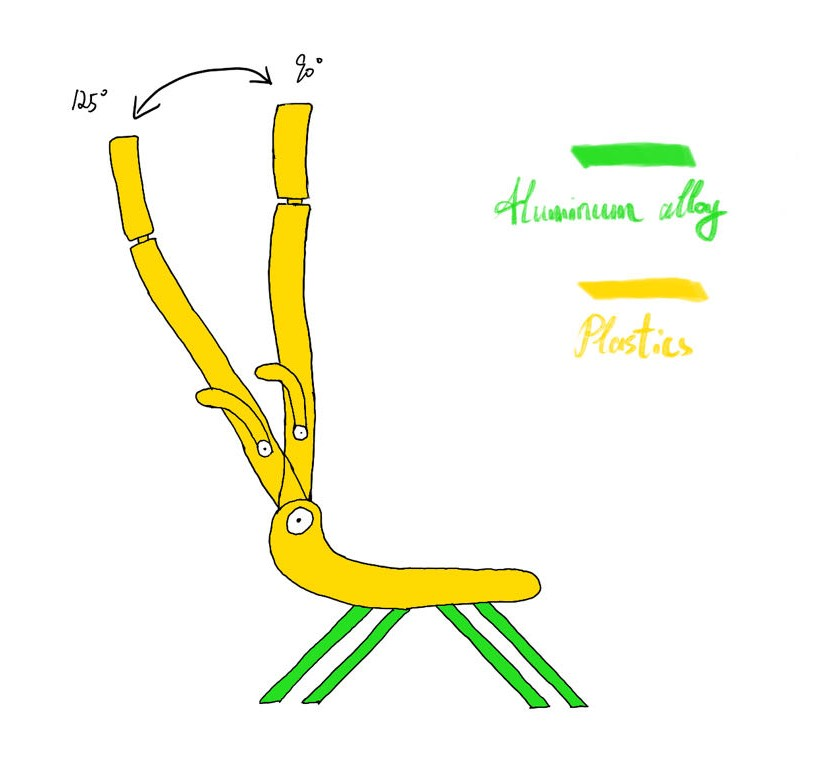
\includegraphics[width=0.6\textwidth]{images/Seat frame.jpg}
    \caption{Seat frame (the support legs are not shown completely in the figure)}
    \label{fig:frame}
\end{figure}


\subsection{Seat Assembly}
The seat assembly, shown in Figure \ref{fig:seat-assembly}, comprises the cover and cushions. The cover, crafted from polyurethane leather, is endowed with waterproof, oil-proof, easy-to-clean features, and outstanding durability. The cushion is composed of superior-quality polyurethane foam that offers passengers excellent support and comfort over extended flights. To generate a peaceful and comfortable ambiance, blue is presumed to be the chosen color for the cover, but airline companies can specify a different color scheme according to their preferences. The cover and cushions come pre-assembled and can be effortlessly affixed to the seat via specialized button-like connections and locking mechanisms, as illustrated in Figure \ref{fig:seat-connection}.

\begin{figure}[!htp]
    \centering
    \includegraphics[width=0.8\textwidth]{images/Seat assembly.png}
    \caption{Seat assembly}
    \label{fig:seat-assembly}
\end{figure}

\begin{figure}[!htp]
    \centering
    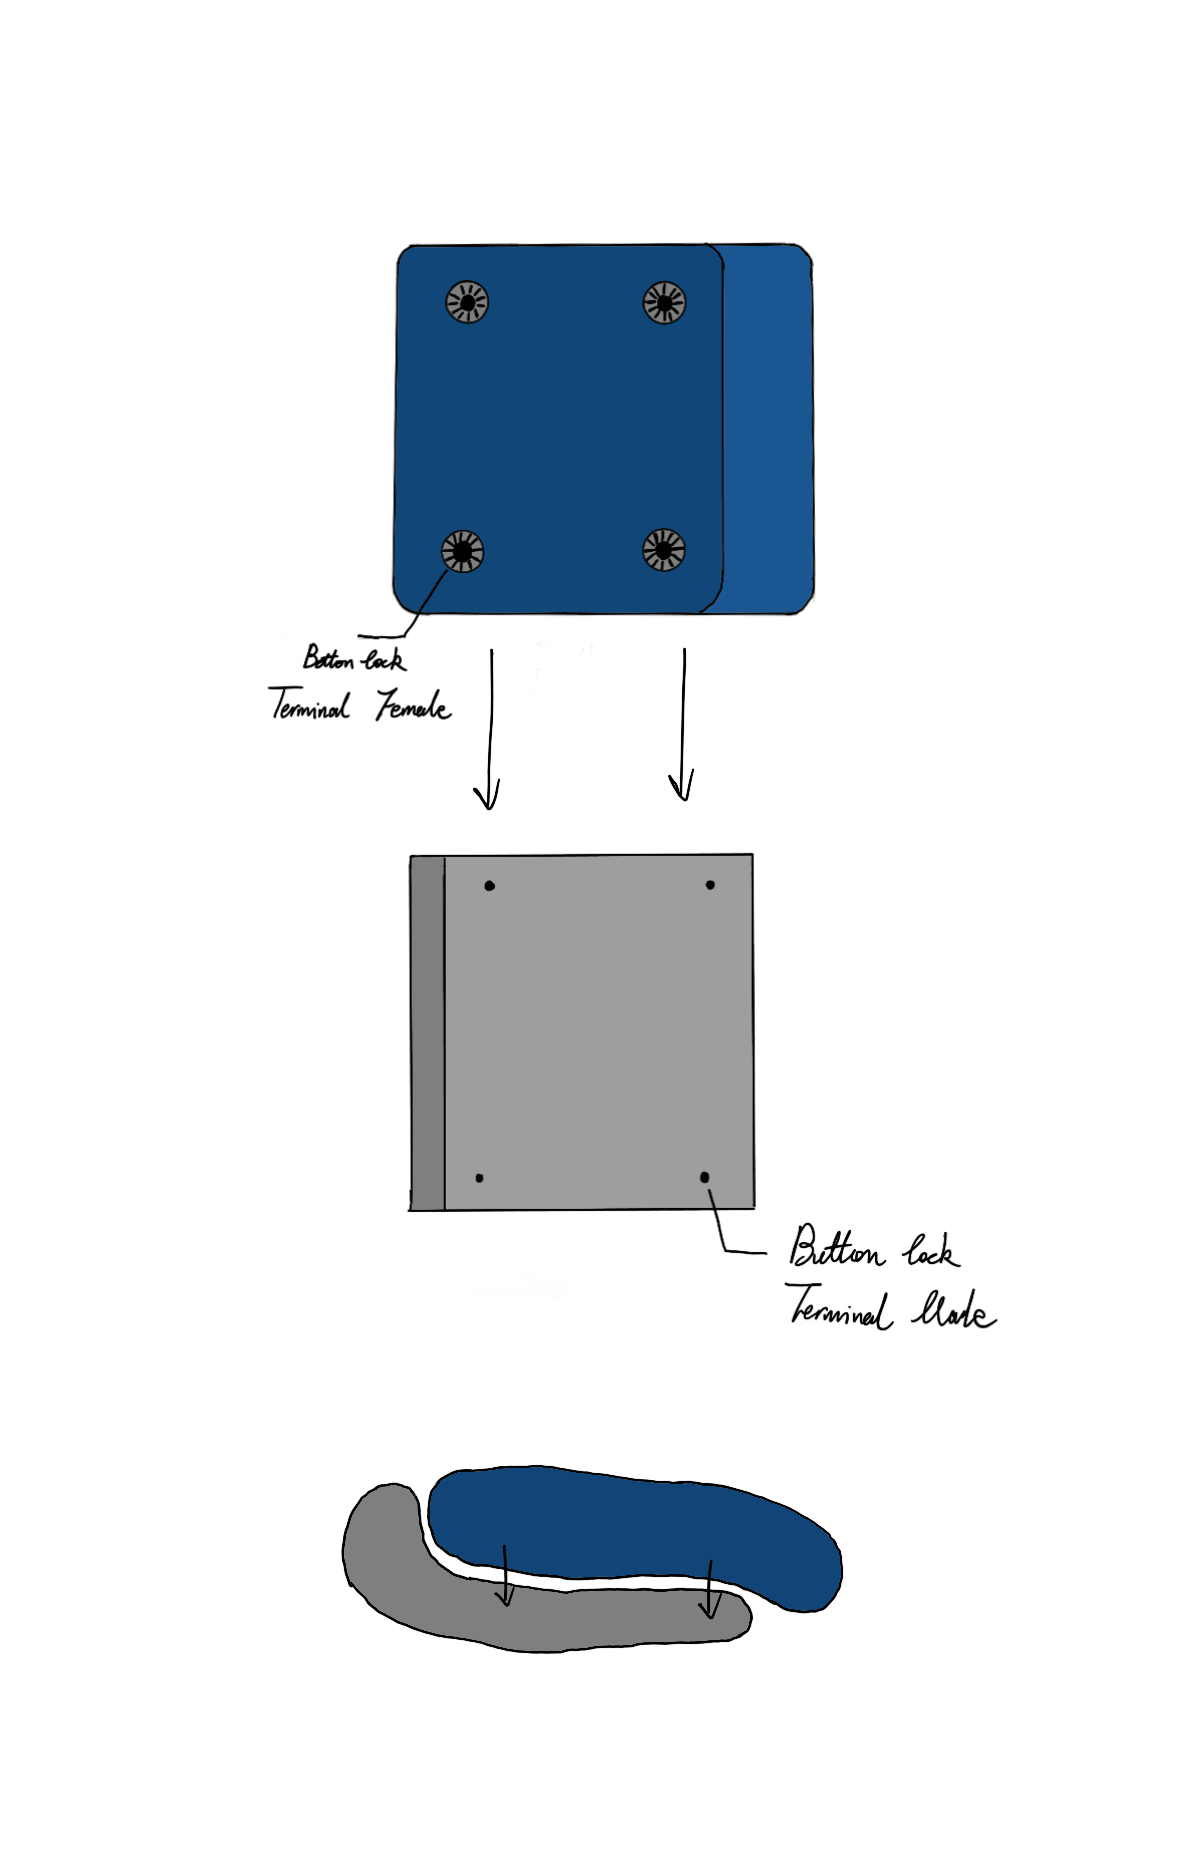
\includegraphics[width=0.8\textwidth]{images/button lock.png}
    \caption{Button-like connections and locking mechanisms on the seat frame and seat assembly and their connection}
    \label{fig:seat-connection}
\end{figure}

\subsection{Headrest Assembly}
The headrest assembly substantially resembles that of the seat; the sole difference is in its size. Consequently, this report does not provide a specific explanation of the headrest assembly.

\subsection{Backrest Assembly}
The backrest assembly substantially resembles that of the seat; the sole difference is in its size. Consequently, this report does not provide a specific explanation of the backrest assembly.

\subsection{Armrests}
A single seat features dual armrests, affording passengers the opportunity to rest their arms individually and comfortably, thereby eliminating the necessity of sharing armrests with adjacent passengers. The armrests, constructed from plastic, exhibit lightweight and durable properties. Additionally, a hinge binds the armrests' root to the seatback, enabling the armrests to be raised, thus allowing for more convenient entry and egress or shared seating accommodations among companions. The armrests are depicted in Figure \ref{fig:armrest-connection}.

\begin{figure}[!htp]
    \centering
    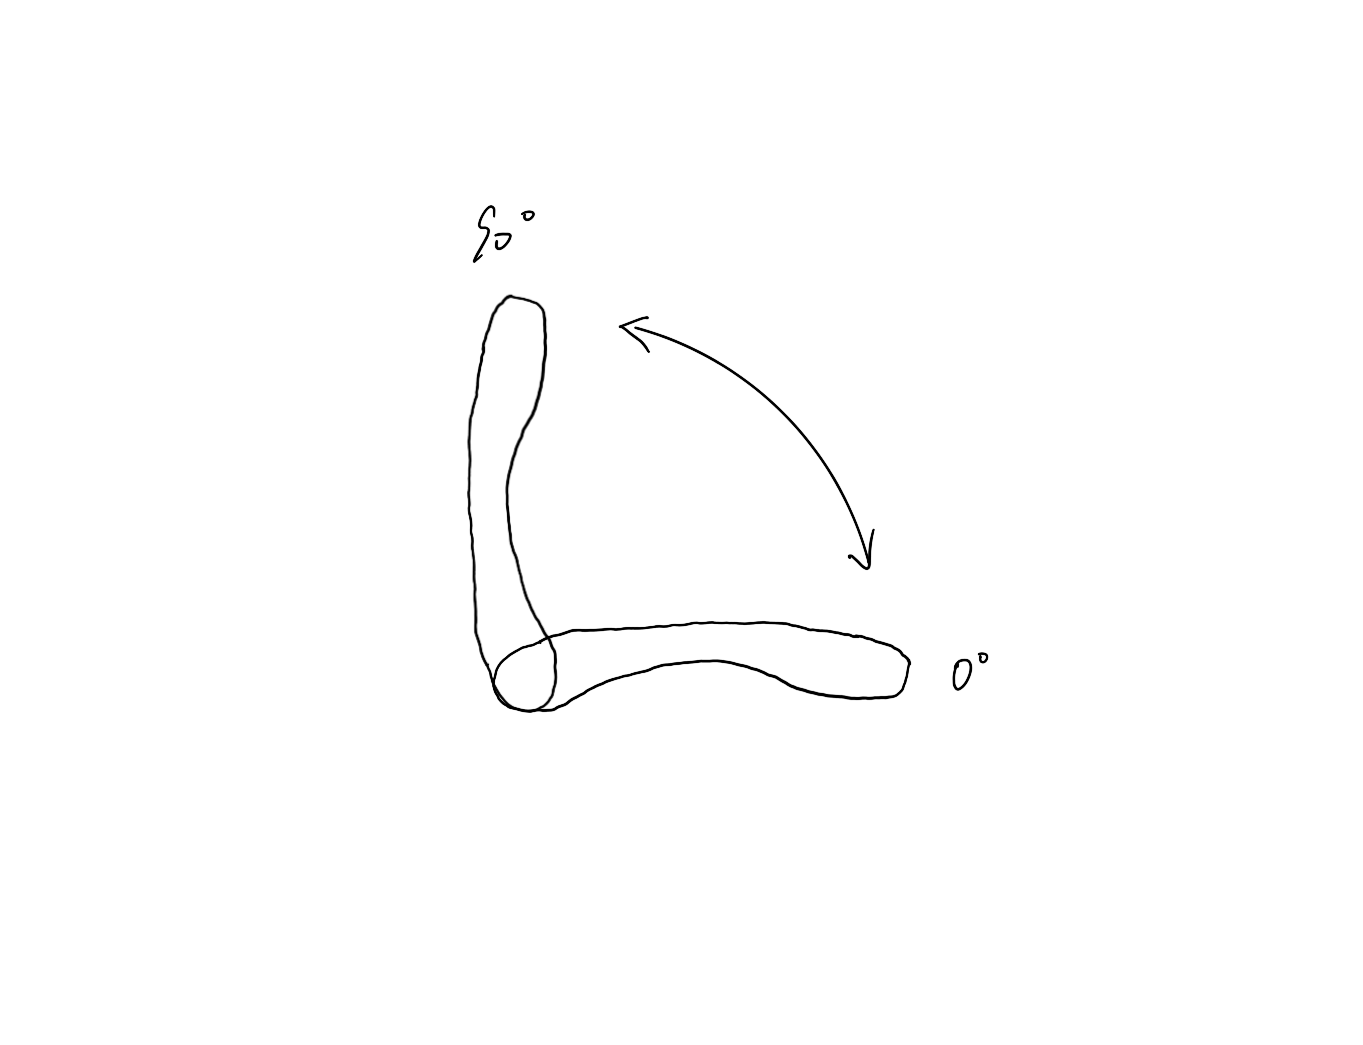
\includegraphics[width=0.8\textwidth]{images/Armrest.png}
    \caption{Armrest (can be raised and lowered for a range of motion of 90 degrees)}
    \label{fig:armrest-connection}
\end{figure}

\subsection{Foldable Desk Assembly}
Constructed from lightweight and rigid plastic, the foldable desk serves to provide passengers with a practical platform for stowing personal effects or consuming meals. Boasting a maximum load-bearing capacity of 5 kg, passengers will be duly informed of the reduced weight limit of 4 kg in the interests of safety. Articulated via a hinge affixed to the backrest, the table may be folded upwards or downwards at will. A single swivel latch, positioned on the desk's lower periphery, serves to secure the table in a folded configuration, retaining it against the backrest when not in use. Upon opening this latch, the desk descends by means of gravity to a level position in front of the passenger. Figure \ref{fig:desk-connection} illustrates the design of the foldable desk.

\begin{figure}[!htp]
    \centering
    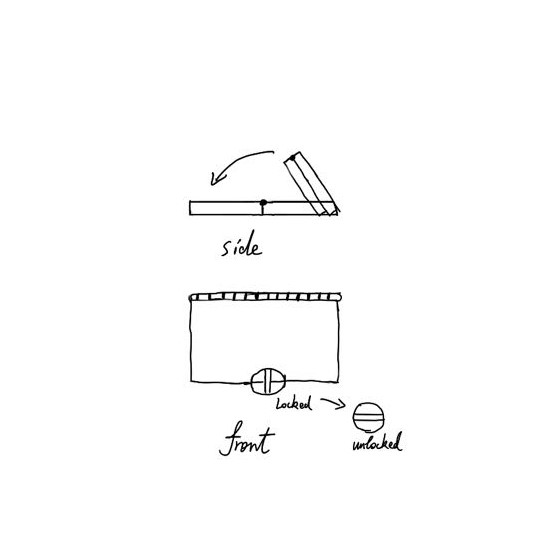
\includegraphics[width=0.8\textwidth]{images/desk.jpg}
    \caption{Foldable desk assembly}
    \label{fig:desk-connection}
\end{figure}


\subsection{Connections and Fasteners}
In the current prototype, the integrity of the structure relies significantly on the efficacy of the connections and fasteners employed. Screws serve as an essential component, securing the legs to the floor and fastening the seat frame to maintain stability. Hinges, on the other hand, are implemented in all rotational joints, including those between the backrest and seat frame, armrest and seat frame, and foldable desk and backrest. In addition, button-like connections are integrated into the design to facilitate the attachment of the seat assembly to the seat frame, enabling straightforward replacements of covers and cushions and simplifying the seat's cleaning process. This innovative design feature holds significant potential for enhancing the functionality of the seat.